\documentclass[a4paper,11pt]{article}

\usepackage[utf8]{inputenc}
\usepackage{graphicx}
\usepackage{caption}
\usepackage{subcaption}
\usepackage{float}
\usepackage{amsmath}
\usepackage{pgfplots}
\usepackage{ffcode}
\usepackage{booktabs}
\usepackage{listings}
\usepackage{xcolor}
\usepackage{listings}
\usepackage{array}
\usepackage{tikz}
\usepackage{algorithm}
\usepackage{algpseudocode}
\usetikzlibrary{calc,patterns,angles,quotes}

\pgfplotsset{compat=1.18} 

\begin{document}
	
\title{
	\textbf{Quadson}
}
\author{Ying Pei Lin}
\date{Spring 2025}
\maketitle

\section*{Introduction}

Quadson is a 3D printed quadruped robot designed as a platform for exploring advanced robotic motion and control.
This document includes its forward kinematics, inverse kinematics, differential kinematics and expands to body kinematics.
Following this analysis, we will introduce the process of performing simultion in Pybullet and using deep
reinforcement learning to improve the robot's control and performance.

\section*{Forward Kinematics}

For each leg of the robot, we define the reference frame with its origin at point $p_1$. 
Two motors are positioned at $p_1$ and $p_5$ respectively, and the third motor
connected to the entire leg assembly, controls the rotation around x axis. The remaining joints in the leg are all passive.

\begin{center}
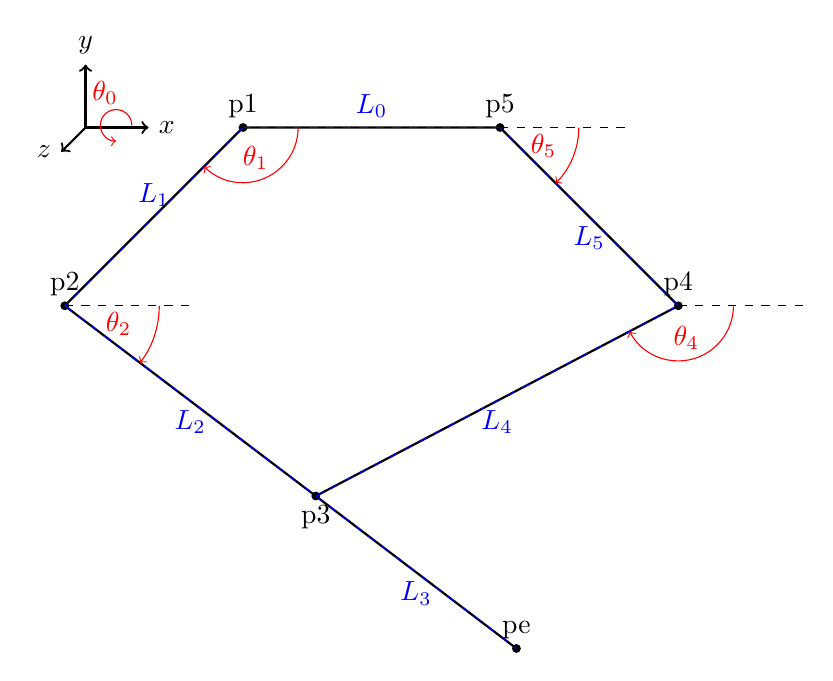
\begin{tikzpicture}[scale=0.4]
	% Points
	\coordinate (p1) at (0,0);
	\coordinate (p2) at (-5.66,-5.66);
	\coordinate (p2_hori) at (-1.66,-5.66);
	\coordinate (p3) at (2.31,-11.70);
	\coordinate (pe) at (8.68,-16.54);
	\coordinate (p4) at (13.82,-5.66);
	\coordinate (p4_hori) at (17.82,-5.66);
	\coordinate (p5) at (8.16,0);
	\coordinate (p5_hori) at (12.16,0);

	% Lines
	\draw[thick] (p1) -- (p2) -- (p3) -- (p4) -- (p5) -- (p1);
	\draw[thick] (p3) -- (pe);
	\draw[dashed] (p2) -- (p2_hori);
	\draw[dashed] (p4) -- (p4_hori);
	\draw[dashed] (p5) -- (p5_hori);
	
	% Axis
	\draw[thick,->] (-5,0,0) -- (-3,0,0) node[right] {$x$};
	\draw[thick,->] (-5,0,0) -- (-5,2,0) node[above] {$y$};
	\draw[thick,->] (-5,0,0) -- (-5,0,2) node[left] {$z$};
	\draw[red,->] (-3.8,-0.2,-0.7) arc[start angle=0,end angle=270,radius=0.5cm] node[midway,above] {$\theta_0$};

	% Point tags
	\foreach \p in {p1, p2, pe, p4, p5} {
			\fill[black] (\p) circle (4pt);
			\node[above] at (\p) {\p};
	}
	\fill[black] (p3) circle (4pt);
	\node[below] at (p3) {p3};

	% Length tags
	\draw[blue, dashed] (p1) -- (p5) node[midway, above] {$L_{0}$};
	\draw[blue, dashed] (p1) -- (p2) node[midway, above] {$L_{1}$};
	\draw[blue, dashed] (p2) -- (p3) node[midway, below] {$L_{2}$};
	\draw[blue, dashed] (p3) -- (pe) node[midway, below] {$L_{3}$};
	\draw[blue, dashed] (p3) -- (p4) node[midway, below] {$L_{4}$};
	\draw[blue, dashed] (p4) -- (p5) node[midway, below] {$L_{5}$};

	% Angle tags
	\pic [draw=red, text=red, <-, "$\theta_1$", angle radius=0.7cm] {angle=p2--p1--p5};
	\pic [draw=red, text=red, <-, "$\theta_2$", angle radius=1.2cm] {angle=p3--p2--p2_hori};
	\pic [draw=red, text=red, <-, "$\theta_4$", angle radius=0.7cm] {angle=p3--p4--p4_hori};
	\pic [draw=red, text=red, <-, "$\theta_5$", angle radius=1cm] {angle=p4--p5--p5_hori};
\end{tikzpicture}
\end{center}

The following algorithm takes the angle of three motors as input and computes the position of the end effector.
The process incorporates several safety check, prevent configurations that could potentially damage the mechanism.

\begin{algorithm}[H]
	\caption{Compute Leg End-Point}
	\begin{algorithmic}[1]
			\Require Motor angles $\theta_0, \theta_1, \theta_5$
			\State Perform safety checks and limit angles
			\State Compute initial 2D joint positions:
			\[
				p_2 = (L_1 \cos \theta_1, -L_1 \sin \theta_1), \quad
				p_5 = (L_0, 0), \quad
				p_4 = p_5 + (L_5 \cos \theta_5, -L_5 \sin \theta_5)
			\]
			\State Compute distances:
			\[
					L_{14} = \| p_4 - p_1 \|, \quad
					L_{24} = \| p_4 - p_2 \|
			\]
			\If{$L_{24} < 5$ or $L_{24} > L_2 + L_4$}
					\State Mark as unsafe and return previous endpoint
			\EndIf
			\State Solve for $p_3$ using angles:
			\[
					\theta_2 = \cos^{-1} \left( \frac{L_2^2 + L_{24}^2 - L_4^2}{2 L_2 L_{24}} \right) +
										 \cos^{-1} \left( \frac{L_1^2 + L_{24}^2 - L_{14}^2}{2 L_1 L_{24}} \right) - (\pi - \theta_1)
			\]
			\[
					p_3 = p_2 + L_2 (\cos \theta_2, -\sin \theta_2)
			\]
			\State Compute endpoint:
			\[
					p_e = p_2 + (L_2 + L_3)(\cos \theta_2, -\sin \theta_2)
			\]
			\State Transform to 3D using rotation matrix:
			\[
					R_{\theta_0} =
					\begin{bmatrix}
							1 & 0 & 0 \\
							0 & \cos(-\theta_0) & -\sin(-\theta_0) \\
							0 & \sin(-\theta_0) & \cos(-\theta_0)
					\end{bmatrix}
			\]
			\State Update joint angles and return $p_e$
	\end{algorithmic}
\end{algorithm}

\section*{Inverse Kinematics}

In real world scenarios, controlling position of the end effector to reach to a certain position
is often more pratical than setting the angles directly. For example, to move the end effector along 
a defined trajectory, achieving this by manually adjusting the three motor angles is nearly impossible 
due to the complexity of the joint movements. 

Therefore we need the following algorithm 
to compute the angles of the motor corresponding to a given target position.

\begin{algorithm}[H]
	\caption{Compute Joint Angles from End-Point}
	\begin{algorithmic}[1]
			\Require End-point position $(x, y, z)$
			\State Calculate angle of motor 0:
			\[
				\theta_0 = -\tan^{-1} \left( \frac{z}{-y} \right)
			\]
			\State Translate points from 3D to 2D using rotation matrix:
			\[
				R_{\theta_0} =
					\begin{bmatrix}
							1 & 0 & 0 \\
							0 & \cos(-\theta_0) & -\sin(-\theta_0) \\
							0 & \sin(-\theta_0) & \cos(-\theta_0)
					\end{bmatrix}
			\]
			\[
				\begin{bmatrix} x' \\ y' \\ z' \end{bmatrix} = \text{transformation matrix} \times \begin{bmatrix} x \\ y \\ z \end{bmatrix}
			\]
			\State Calculate angle 1:
			\[
					L_{1e} = \| (x', y') \|, \quad
					\theta_{e15} = \tan^{-1} \left( \frac{-y'}{x'} \right)
			\]
			\[
					\theta_{e12} = \cos^{-1} \left( \frac{L_1^2 + L_{1e}^2 - (L_2 + L_3)^2}{2 L_1 L_{1e}} \right)
			\]
			\[
					\theta_1 = \theta_{e15} + \theta_{e12}
			\]
			\State Compute positions of joints:
			\[
					p_1 = (0, 0), \quad
					p_2 = (L_1 \cos \theta_1, -L_1 \sin \theta_1)
			\]
			\[
					p_3 = \frac{(pe_2d \cdot L_2) + (p_2 \cdot L_3)}{L_2 + L_3}, \quad
					p_5 = (L_0, 0)
			\]
			\State Calculate angle 5:
			\[
				\theta_{350} = \tan^{-1} \left( \frac{-p_3[1]}{L_0 - p_3[0]} \right)
			\]
			\[
					\theta_{354} = \cos^{-1} \left( \frac{L_{35}^2 + L_5^2 - L_4^2}{2 L_{35} L_5} \right), \quad
					L_{35} = \| p_3 - p_5 \|
			\]
			\[
					\theta_5 = \pi - (\theta_{350} + \theta_{354})
			\]
			\State Perform safety checks on angles:
			\State \Return $(\theta_0, \theta_1, \theta_5)$
	\end{algorithmic}
\end{algorithm}

\section*{Differential Kinematics}

To control a quadruped robot's leg smoothly, we employ differential kinematics, which maps joint angular velocities to the linear velocity of the end effector.

\subsection*{Kinematic Relation}

Let $\boldsymbol{\theta} = [\theta_0, \theta_1, \theta_5]^T$ be the motor angles 
and $\dot{\boldsymbol{\theta}} = [\omega_0, \omega_1, \omega_5]^T$ be their angular velocities. 
The linear velocity of the end-effector $\mathbf{v} = [v_x, v_y, v_z]^T$ is given by:

$$
\mathbf{v} = \mathbf{J}(\boldsymbol{\theta}) \cdot \dot{\boldsymbol{\theta}}
$$

Where $\mathbf{J}(\boldsymbol{\theta}) \in \mathbf{R}^{3 \times 3}$ is the Jacobian matrix. 
Due to the complexity of mechanism, the jacobian is computed numerically instead of derive the anatical form.

To find the inverse, the required motor angular velocities for a desired end-effector linear velocity:

$$
\dot{\boldsymbol{\theta}} = \mathbf{J}^{+}(\boldsymbol{\theta}) \cdot \mathbf{v}
$$

Where $\mathbf{J}^+$ is the Moore–Penrose pseudoinverse of $\mathbf{J}$.

\begin{algorithm}[H]
	\caption{Compute Joint Velocities from End-Effector Velocity}
	\begin{algorithmic}[1]
		\Require End-effector velocity $\mathbf{v} = [v_x, v_y, v_z]^T$
		\Ensure Joint angular velocities $\dot{\boldsymbol{\theta}} = [\omega_0, \omega_1, \omega_2]^T$
		\State Read current joint angles $\boldsymbol{\theta}$
		\State Compute forward kinematics to get $\mathbf{p} = f(\boldsymbol{\theta})$
		\State Compute numerical Jacobian $\mathbf{J} \in \mathbf{R}^{3 \times 3}$
		\State Compute pseudoinverse $\mathbf{J}^{+}$
		\State Compute $\dot{\boldsymbol{\theta}} = \mathbf{J}^{+} \cdot \mathbf{v}$
		\State \Return $\dot{\boldsymbol{\theta}}$
	\end{algorithmic}
\end{algorithm}

\subsection*{Numerical Jacobian Approximation}

Due to the difficulty in analytically deriving $\mathbf{J}(\boldsymbol{\theta})$, we use the numerical finite difference method:

$$
\mathbf{J}_{:,i} = \frac{f(\boldsymbol{\theta} + \delta \cdot \mathbf{e}_i) - f(\boldsymbol{\theta})}{\delta}
$$

Where $f(\boldsymbol{\theta})$ is the forward kinematics function, $\delta$ is a small perturbation and 
$\mathbf{e}_i$ is a unit vector along the $i$-th motor axis.

\subsection*{Practical Considerations}

\begin{itemize}
  \item Angular velocity of the end-effector ($\omega_x, \omega_y, \omega_z$) is ignored because the foot contact does not require rotational control in this context.
  \item The Jacobian is updated continuously as $\boldsymbol{\theta}$ changes during motion even though the given linear velocity remain the same.
\end{itemize}

\section*{Body Kinematics}

Given the positions of the end-effectors (feet) in the world frame and the orientation of the body, the goal is to compute the foot positions expressed in the local shoulder frames of the robot.

Coordinate Frames: 
\begin{itemize}
	\item \textbf{World Frame (W)} - Global reference frame.
	\item \textbf{Body Frame (B)} - Attached to the robot's center.
	\item \textbf{Shoulder Frame (S)} - Local frame attached to each leg's shoulder joint.
\end{itemize}

\subsubsection*{Transformation Matrices}
Each coordinate transformation is represented using a 4x4 homogeneous transformation matrix, composed of a rotation matrix $R$ and a translation vector $p$:

\[
T = \begin{bmatrix}
R & p \\
0 & 1
\end{bmatrix}
\]

To transform a point from the shoulder frame to the world frame:

\[
T_s = T_b T_s^b
\]

Where:
\begin{itemize}
    \item $T_b$: Transformation from body frame to world frame.
    \item $T_s^b$: Transformation from shoulder frame to body frame (fixed).
    \item $T_s$: Transformation from shoulder frame to world frame.
\end{itemize}

To express a point $p^w$ in the world frame as $p^s$ in the shoulder frame:

\[
T_w^s = T_s^{-1}, \quad p^s = T_w^s p^w
\]

\subsubsection*{Algorithm}
\begin{algorithm}[H]
\caption{Compute Foot Position in Shoulder Frame}
\begin{algorithmic}[1]
\State \textbf{Input:} Foothold positions $p^w_i$, body orientation $(roll, pitch, yaw)$
\State Compute $T_b \gets$ transformation from body frame to world frame
\For{each leg $i$}
    \State Get shoulder-to-body transform $T_{s_i}^b$ (predefined by geometry)
    \State Compute $T_{s_i} = T_b \cdot T_{s_i}^b$
    \State Compute inverse $T_w^{s_i} = T_{s_i}^{-1}$
    \State Project world foot point into shoulder frame:
    \[
    p_i^s = T_w^{s_i} p_i^w
    \]
\EndFor
\State \textbf{Output:} Foot positions $p_i^s$ in shoulder frames
\end{algorithmic}
\end{algorithm}

\subsubsection*{Concept Summary}
\begin{itemize}
	\item The robot body's pose is updated in the world using the orientation (roll, pitch, yaw).
	\item Each leg has a fixed shoulder position in the body frame and a defined orientation relative to the body.
	\item By chaining transformations from the world frame to the shoulder frame, we project world-coordinates of the feet into each leg's local frame.
\end{itemize}

\section*{Locomotion}

Locomotion control is crucial for quadruped robots to enable them to move efficiently. The motion of the robot depends on the type of gait used, and different gaits have different characteristics such as step height, length, and timing.

The following algorithm is used to calculate the phases of each leg and the corresponding end-effector points for locomotion based on the gait type.

\begin{algorithm}[H]
	\caption{Locomotion Phase Calculation}
	\begin{algorithmic}[1]
		\Require Gait type: \texttt{gait\_type} (must be one of 'walk', 'trot', 'pace', 'bound', or 'gallop')
		\State Set constants based on \texttt{gait\_type}:
		\[
			\text{PHASE\_OFFSETS}, \text{CYCLE\_TIMES}, \
			\quad \text{DUTY\_FACTORS}, \quad \text{STEP\_HEIGHTS}, \
			\quad \text{STEP\_LENGTHS}
		\]
		\State Initialize class with the selected \texttt{gait\_type}
		\State Calculate the current phase of each leg based on the current time:
		\[
			\text{cycle\_progress} = \frac{\text{time} \% \text{cycle\_time}}{\text{cycle\_time}}
		\]
		\For{each leg in the robot's leg configuration}
			\State Calculate phase based on cycle progress:
			\[
				\text{phase\_dict[leg\_name]} = (\text{cycle\_progress} + \text{phase\_offset}) \% 1.0
			\]
		\EndFor
		\State \Return phase dictionary: \texttt{phase\_dict}
	\end{algorithmic}
\end{algorithm}

Once the phase of each leg is determined, the next step is to calculate the end-effector (foot) positions for each leg. The position is calculated differently for the stance and swing phases of each gait cycle.

\begin{algorithm}[H]
	\caption{End-Effector Points Calculation}
	\begin{algorithmic}[1]
		\Require Current time: \texttt{time}
		\State Get current phase for each leg using \texttt{get\_current\_phase(time)}
		\For{each leg in the robot's leg configuration}
			\If{phase of the leg is in the stance phase (i.e., less than \texttt{duty\_factor})}
				\State Interpolate between the stance start and end points:
				\[
					\text{p\_start} = (start\_x, base\_y), \quad \text{p\_end} = (start\_x + direction \times \text{step\_length}, base\_y)
				\]
				\[
					p = \text{p\_start} + (\text{p\_end} - \text{p\_start}) \times \frac{\text{phase}}{\text{duty\_factor}}
				\]
				\State Set \texttt{x, y} coordinates based on interpolation
			\Else
				\State Interpolate using cubic Bezier curve for swing phase:
				\[
					p_0 = (start\_x + direction \times \text{step\_length}, base\_y), \quad
					p_1 = (start\_x + direction \times \text{step\_length}/2, base\_y + \text{step\_height}), \quad
					p_2 = (start\_x, base\_y + \text{step\_height}/2), \quad p_3 = (start\_x, base\_y)
				\]
				\[
					(x, y) = \text{cubic\_bezier}(t, p_0, p_1, p_2, p_3)
				\]
			\EndIf
			\State Set \texttt{ee\_points[leg\_name]} to the calculated coordinates
		\EndFor
		\State \Return end-effector points: \texttt{ee\_points}
	\end{algorithmic}
\end{algorithm}

The cubic Bezier curve is used for the swing phase to smoothly interpolate the leg's motion. The following formula is used to calculate the position on the cubic Bezier curve.

\begin{algorithm}[H]
	\caption{Cubic Bezier Curve}
	\begin{algorithmic}[1]
		\Require Interpolation factor: \texttt{t}, Control points: \texttt{p0, p1, p2, p3}
		\State Define the control points as a matrix:
		\[
			\text{points} = \begin{bmatrix} p_0 \\ p_1 \\ p_2 \\ p_3 \end{bmatrix}
		\]
		\State Define the Bernstein coefficients for the cubic curve:
		\[
			\text{coeffs} = \begin{bmatrix} (1-t)^3 & 3(1-t)^2t & 3(1-t)t^2 & t^3 \end{bmatrix}
		\]
		\State Calculate the position on the curve:
		\[
			(x, y) = \text{coeffs} \times \text{points}
		\]
		\State \Return position \texttt{(x, y)}
	\end{algorithmic}
\end{algorithm}

\section*{Simulation}

\section*{Deep Reinforcement Learning}

\section*{Conclusion}

\end{document}